\documentclass[border=3mm,tikz,preview]{standalone}
\usepackage[utf8]{inputenc}
\usepackage{amsmath,amssymb,amsfonts}
\usepackage{graphicx}
\usepackage{tikz}
\usetikzlibrary{shapes.geometric, arrows.meta, positioning, shadows, calc, fit, backgrounds}
\usepackage{xcolor}
\begin{document}

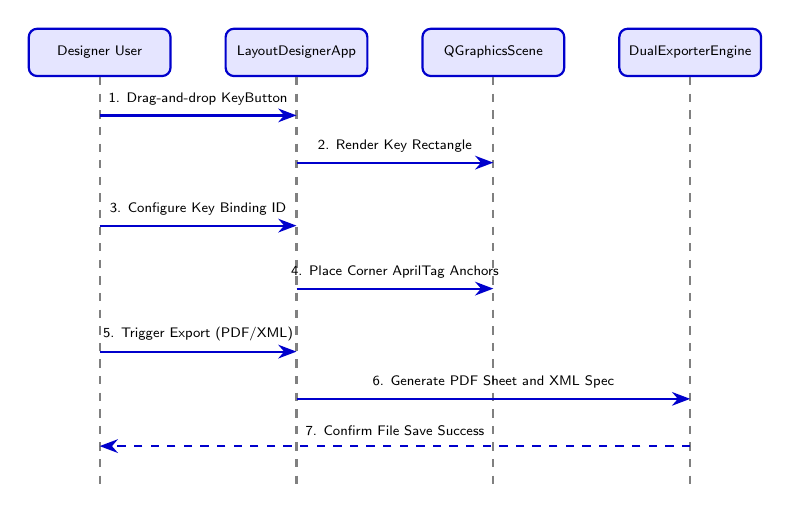
\begin{tikzpicture}[
    lifeline/.style = {draw=black!50, dashed, thick},
    entity/.style = {rectangle, draw=blue!80!black, fill=blue!10!white, thick, rounded corners=3pt, align=center, font=\sffamily\tiny, minimum width=1.8cm, minimum height=0.6cm},
    msg/.style = {draw=blue!80!black, ->, >=Stealth, thick, font=\sffamily\tiny},
    reply/.style = {draw=blue!80!black, ->, >=Stealth, dashed, thick, font=\sffamily\tiny}
]

% Entities
\node (user) [entity] at (0, 0) {Designer User};
\node (gui) [entity] at (2.5, 0) {LayoutDesignerApp};
\node (canvas) [entity] at (5.0, 0) {QGraphicsScene};
\node (exporter) [entity] at (7.5, 0) {DualExporterEngine};

% Lifelines
\draw [lifeline] (user) -- (0, -5.5);
\draw [lifeline] (gui) -- (2.5, -5.5);
\draw [lifeline] (canvas) -- (5.0, -5.5);
\draw [lifeline] (exporter) -- (7.5, -5.5);

% Messages
\draw [msg] (0, -0.8) -- node[above]{1. Drag-and-drop KeyButton} (2.5, -0.8);
\draw [msg] (2.5, -1.4) -- node[above]{2. Render Key Rectangle} (5.0, -1.4);
\draw [msg] (0, -2.2) -- node[above]{3. Configure Key Binding ID} (2.5, -2.2);
\draw [msg] (2.5, -3.0) -- node[above]{4. Place Corner AprilTag Anchors} (5.0, -3.0);
\draw [msg] (0, -3.8) -- node[above]{5. Trigger Export (PDF/XML)} (2.5, -3.8);
\draw [msg] (2.5, -4.4) -- node[above]{6. Generate PDF Sheet and XML Spec} (7.5, -4.4);
\draw [reply] (7.5, -5.0) -- node[above]{7. Confirm File Save Success} (0, -5.0);

\end{tikzpicture}

\end{document}
